%!TEX root = ../preamble.tex

\section{Results}
\label{sec:results}

\subsection{Experiments with the convolutional neural network}


\subsubsection{Feature maps}
The feature maps shown on figure \ref{fig:featuremaps} are visualised by scaling the output range of $[0,1]$ of every neuron linearly to the grey scale range of $[0,255]$. The leftmost column of feature maps are from the first convolutional layer, and the rightmost is the input to the fully connected layers. As a convolutional layer takes a depth slice of all the previous feature maps as input, their is no apparent connection between the visualised output of the max pooling layer and the following result of the convolutional layer.

\begin{figure}[H]
	\begin{scriptsize}
		\sffamily
		\def\svgwidth{\textwidth}
		\input{img/featuremaps.pdf_tex}
	\end{scriptsize}
	\caption{A small subset of the feature maps produced from running a training example from the lightened arena through the visual partitioning classification deep convolutional neural network. The feature maps highlight the position of the target.}
	\label{fig:featuremaps}
\end{figure}

%Shallow vs deep
%No light vs light

%%!TEX root = ../preamble.tex

\pgfplotstableread{data/nolight-angular-shallow.dat}{\nolightAngularShallow}
\pgfplotstableread{data/nolight-angular-deep.dat}{\nolightAngularDeep}

\begin{figure}[H]
\begin{tikzpicture}[scale=1]
	\begin{axis}[
			title=Score over iterations,
			xlabel=Iterations,
			ylabel=Score,
			xmin = -640,
			xmax = 16640,
			restrict x to domain=0:16000,
			xticklabel style={rotate=30},
			minor x tick num=1,
			legend pos=north east,
		]
		\addplot+ [cred, mark=none] table [x={iteration}, y={score}] {\nolightAngularShallow};
		\addlegendentry{Shallow architecture}
		\addplot+ [cblue, mark=none] table [x={iteration}, y={score}] {\nolightAngularDeep};
		\addlegendentry{Deep architecture}
	\end{axis}
\end{tikzpicture}
\caption{Training convolutional neural networks using angular regression without visual distortion}
\end{figure} %DONE
%%!TEX root = ../preamble.tex

\pgfplotstableread{data/light-angular.dat}{\lightAngular}
\begin{figure}[H]
\begin{tikzpicture}[scale=1]
	\begin{axis}[
			xlabel=Iterations,
			ylabel=Score,
			xmin = -640,
			xmax = 16640,
			restrict x to domain=0:16000,
			xticklabel style={rotate=30},
			minor x tick num=1,
		]
		\addplot+ [red, mark=none] table [x={iteration}, y={score}] {\lightAngular};
	\end{axis}
\end{tikzpicture}
\caption{Training of a deep convolutional network to detect angles and distance with light}
\end{figure}


%%!TEX root = ../preamble.tex

\pgfplotstableread{data/nolight-vpr-shallow.dat}{\nolightVPRShallow}
\pgfplotstableread{data/nolight-vpr-deep.dat}{\nolightVPRDeep}

\begin{figure}[H]
\begin{tikzpicture}[scale=1]
	\begin{axis}[
			title=Score over iterations,
			xlabel=Iterations,
			ylabel=Score,
			xmin = -480,
			xmax = 12480,
			restrict x to domain=0:12000,
			xticklabel style={rotate=30},
			legend pos=north east,
		]
		\addplot+ [cred, mark=none] table [x={iteration}, y={score}] {\nolightVPRShallow};
		\addlegendentry{Shallow architecture}
		\addplot+ [cblue, mark=none] table [x={iteration}, y={score}] {\nolightVPRDeep};
		\addlegendentry{Deep architecture}
	\end{axis}
\end{tikzpicture}
\caption{Training convolutional neural networks using VPR without visual distortion}
\end{figure} %DONE
%%!TEX root = ../preamble.tex

\pgfplotstableread{data/light-vpr-shallow.dat}{\lightVPRShallow}
\pgfplotstableread{data/light-vpr-deep.dat}{\lightVPRDeep}

\begin{figure}[H]
\begin{tikzpicture}[scale=1]
	\begin{axis}[
			title=Score over iterations,
			xlabel=Iterations,
			ylabel=Score,
			xmin = -480,
			xmax = 12480,
			restrict x to domain=0:12000,
			xticklabel style={rotate=30},
			legend pos=north east,
		]
		\addplot+ [cred, mark=none] table [x={iteration}, y={score}] {\lightVPRShallow};
		\addlegendentry{Shallow architecture}
		\addplot+ [cblue, mark=none] table [x={iteration}, y={score}] {\lightVPRDeep};
		\addlegendentry{Deep architecture}
	\end{axis}
\end{tikzpicture}
\caption{Training convolutional neural networks using VPR with visual distortion}
\end{figure} %DONE

%%!TEX root = ../preamble.tex






\definecolor{cpurple}{HTML}{BA6FB6}
\definecolor{corange}{HTML}{FDAE61}
\definecolor{cgreen}{HTML}{ABDDA4}
\definecolor{cblue}{HTML}{2B83BA}

\begin{figure}[H]
\centering
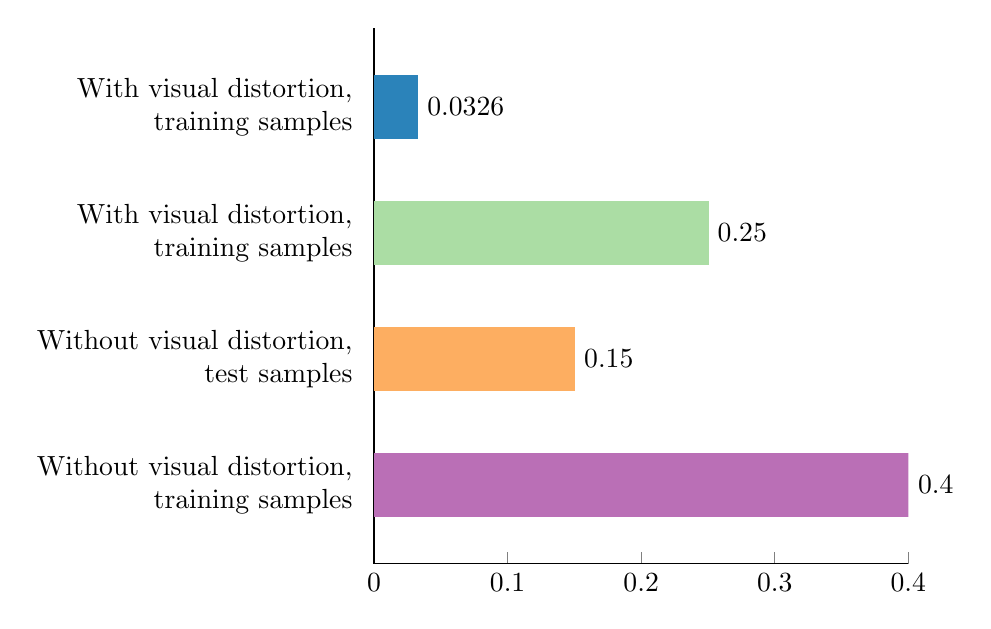
\begin{tikzpicture}
\begin{axis}[
    xbar=0pt,
    /pgf/bar shift=0pt,
    legend style={
    legend columns=4,
        at={(xticklabel cs:0.5)},
        anchor=north,
        draw=none
    },
    ytick={0,...,3},
    ytick style={draw=none},
    axis y line*=none,
    axis x line*=bottom,
    xtick={0,0.1,...,0.5},
    width=.69\textwidth,
    bar width=8mm,
	yticklabels={	{Without visual distortion,\\training samples}, 
						{Without visual distortion,\\test samples}, 
						{With visual distortion,\\training samples}, 
						{With visual distortion,\\training samples}, 
	},
	yticklabel style={align=right},
    xmin=0,
    xmax=0.4,
    area legend,
    y=16mm,
    enlarge y limits={abs=0.625},
    nodes near coords,
    every node near coord/.style={/pgf/number format/fixed, /pgf/number format/precision=5, text=black},
    every axis plot/.append style={fill}
]
\addplot[cpurple] coordinates {(0.400,0)};
\addplot[corange] coordinates {(0.150,1)};
\addplot[cgreen] coordinates {(0.250,2)};
\addplot[cblue] coordinates {(0.0326,3)};
\end{axis}  
\end{tikzpicture}
\caption{X}
\label{fig:stats}
\end{figure}


















































%!TEX root = ../preamble.tex

\hspace{-8mm}
\begin{figure}[H]
\begin{tikzpicture}
\begin{axis}[
	width=0.67\textwidth,
	height=7cm,
	enlarge y limits={abs=0.5},
	xmin=0,
	xmax=100,
	axis y line*=none,
    axis x line*=bottom,
    xbar,
    reverse legend,
    legend style={at={(0.5,-0.2)},anchor=north},
    yticklabels={
		{Without visual distortion\\shallow topology},
		{Without visual distortion\\deep topology},
		{With visual distortion\\shallow topology},
		{With visual distortion\\deep topology},
	},
	yticklabel style={align=right},
    ytick=data,
    nodes near coords,
    every node near coord/.append style={
		/pgf/number format/fixed zerofill,
		/pgf/number format/precision=2
	},
    ]

% Test set
\addplot [draw=cgreen, fill=cgreen!70] coordinates {
	(97.39,3) % Correct value
	(78.95,2)
	(79.12,1)
	(79.84,0)
};

% Training set
\addplot [draw=cred, fill=cred!70] coordinates {
	(97.38,3) % Correct value
	(77.90,2)
	(79.61,1)
	(78.95,0)
};

\legend{Test set,Training set}
\end{axis}

\end{tikzpicture}
\caption{Accuracy of target detection using angular representation}
\label{fig:angular-acc}
\end{figure}

















































 %NEEDS CORRECT DATA
%!TEX root = ../preamble.tex

\hspace{-8mm}
\begin{figure}[H]
\begin{tikzpicture}
\begin{axis}[
	width=0.67\textwidth,
	height=5cm,
	enlarge y limits={abs=0.5},
	xmin=0,
	xmax=0.0021,
	axis y line*=none,
    axis x line*=bottom,
    xbar,
    reverse legend,
    legend style={at={(0.5,-0.1)},anchor=north},
    yticklabels={
		{Mean horizontal error},
		{Mean vertical error},
		{Mean distance error},
	},
	yticklabel style={align=right},
    ytick=data,
	xtick style={draw=none},	
    xticklabels={,,,,,},
    nodes near coords,
    every node near coord/.append style={
		/pgf/number format/fixed zerofill,
		/pgf/number format/precision=6
	},
    ]

\addplot [draw=cgreen, fill=cgreen!70] coordinates {
	(0.001243,3)
	(0.002089,2)
	(0.001004,1)
%	(97.23,0)
};
\addplot [draw=cred, fill=cred!70] coordinates {
	(0.002100,3)
	(0.001324,2)
	(0.001350,1)
%	(97.23,0)
};

\legend{Test set,Training set}
\end{axis}

\end{tikzpicture}
\caption{Angular accuracy without visual distortion}
\label{fig:angular-acc}
\end{figure}
















































 %NEEDS CORRECT DATA